\documentclass[12pt,a4paper]{article}
\usepackage{iftex}
\ifPDFTeX
    \usepackage[utf8]{inputenc}
    \usepackage[T1]{fontenc}
    \usepackage{mathpazo}
\else
    \usepackage{fontspec}
    \setmainfont{Times New Roman}
\fi
\usepackage[brazilian]{babel}
\usepackage{amsmath, amssymb, amsthm}
\usepackage[linesnumbered,ruled,vlined,portuguese]{algorithm2e}
\usepackage{listings}
\usepackage{booktabs}
\usepackage{geometry}
\usepackage{float}
\usepackage{xcolor}
\usepackage{setspace}
\usepackage{graphicx}
\usepackage[colorlinks=true, linkcolor=blue, urlcolor=blue, citecolor=blue]{hyperref}

\geometry{margin=2.5cm}
\onehalfspacing

\definecolor{codebg}{rgb}{0.96,0.96,0.96}
\definecolor{codekey}{rgb}{0.0,0.4,0.8}
\definecolor{codestr}{rgb}{0.6,0.1,0.1}
\definecolor{codecom}{rgb}{0.4,0.6,0.4}

\lstset{
    backgroundcolor=\color{codebg},
    commentstyle=\itshape\color{codecom},
    keywordstyle=\bfseries\color{codekey},
    stringstyle=\color{codestr},
    basicstyle=\ttfamily\footnotesize,
    breaklines=true,
    numbers=left,
    numberstyle=\tiny\color{gray},
    frame=single,
    rulecolor=\color{lightgray},
    captionpos=b,
    tabsize=4
}

\title{
    \vspace{-1cm}
    \begin{center}
        \Large \textbf{Universidade Federal do Ceará -- UFC} \\
        \large Departamento de Computação \\
        \vspace{1cm}
        \Huge \textbf{Métodos Numéricos II} \\
        \vspace{0.5cm}
        \Large \textit{Relatório da Unidade 5: Problemas de Valor de Contorno (PVC)}
    \end{center}
}
\author{
    Nicolas Wallace Amorim Perote -- Matrícula: 566512 \\
    Samyra Vitória Lima de Almeida -- Matrícula: 521240
}
\date{\today}

\begin{document}

\maketitle
\tableofcontents
\newpage

%==========================================================
\section{Introdução}
%==========================================================
A resolução de Equações Diferenciais Ordinárias com condições impostas \emph{simultaneamente em pontos distintos} do domínio configura um Problema de Valor de Contorno (PVC). Ao contrário dos PVIs da Unidade~4 — onde o estado inicial propaga a solução para frente no tempo —, num PVC as restrições nas fronteiras $x=a$ e $x=b$ acoplam todos os graus de liberdade internos, exigindo a montagem e resolução de um sistema linear \emph{global}.

O PVC linear genérico estudado nesta unidade assume a forma
\begin{equation}
    c_2\,u'' + c_1\,u' + c_0\,u = f(x), \qquad u(a) = \alpha,\quad u(b) = \beta.
\end{equation}
Foram implementadas três abordagens distintas, todas expostas na classe unificada \texttt{bvp\_solvers.py}:
\begin{enumerate}
    \item \textbf{MDF 1D} — Diferenças Finitas com diferenças centrais de segunda ordem;
    \item \textbf{MDF 2D} — Diferenças Finitas para a equação de Poisson (iteração Gauss-Seidel);
    \item \textbf{MEF 1D} — Elementos Finitos com elementos lineares de Galerkin.
\end{enumerate}

%==========================================================
\section{Método das Diferenças Finitas em 1D}
%==========================================================
A aproximação central de segunda ordem para as derivadas em nós igualmente espaçados $\Delta x = (b-a)/N$:
\begin{align}
    u''(x_i) &\approx \frac{u_{i-1} - 2u_i + u_{i+1}}{\Delta x^2}, \\
    u'(x_i)  &\approx \frac{u_{i+1} - u_{i-1}}{2\,\Delta x}.
\end{align}
Substituindo na EDO, cada nó interno $i=1,\ldots,N-1$ gera exatamente uma linha de um sistema \emph{tridiagonal}:
\begin{equation}
    \underbrace{\left(\frac{c_2}{\Delta x^2} - \frac{c_1}{2\Delta x}\right)}_{a}\,u_{i-1}
    + \underbrace{\left(-\frac{2c_2}{\Delta x^2} + c_0\right)}_{b}\,u_i
    + \underbrace{\left(\frac{c_2}{\Delta x^2} + \frac{c_1}{2\Delta x}\right)}_{c}\,u_{i+1}
    = f(x_i).
\end{equation}
As condições de Dirichlet $u_0 = \alpha$ e $u_N = \beta$ transferem-se para o vetor do lado direito. O erro de truncamento local é $\mathcal{O}(\Delta x^2)$; portanto, reduzir o passo à metade reduz o erro por um fator de~4.

Na implementação, o sistema tridiagonal é montado via \texttt{scipy.sparse.diags} e resolvido por \texttt{numpy.linalg.solve} após conversão densa — adequado às dimensões tipicamente usadas em exercícios.

\begin{lstlisting}[language=Python, caption={Montagem do sistema tridiagonal no MDF 1D.}]
a_coef = c2 / dx**2 - c1 / (2 * dx)   # sub-diagonal
b_coef = -2 * c2 / dx**2 + c0          # diagonal
c_coef = c2 / dx**2 + c1 / (2 * dx)   # super-diagonal

A = diags([a_coef * ones(n-1), b_coef * ones(n),
           c_coef * ones(n-1)], [-1, 0, 1]).toarray()

rhs[0]  -= a_coef * ua   # condicao de contorno esquerda
rhs[-1] -= c_coef * ub   # condicao de contorno direita

u_int = linalg.solve(A, rhs)
\end{lstlisting}

%==========================================================
\section{Método das Diferenças Finitas em 2D}
%==========================================================
Para a equação de Poisson
\begin{equation}
    \nabla^2 u = f(x, y),
\end{equation}
a estrela de cinco pontos em malha uniforme ($h_x = h_y = h$) aproxima o Laplaciano:
\begin{equation}
    \nabla^2 u_{i,j} \approx \frac{u_{i,j+1} + u_{i,j-1} + u_{i+1,j} + u_{i-1,j} - 4u_{i,j}}{h^2}.
\end{equation}
Isolando $u_{i,j}$:
\begin{equation}
    u_{i,j} = \frac{u_{i,j+1}+u_{i,j-1}+u_{i+1,j}+u_{i-1,j} - h^2 f(x_i,y_j)}{4}.
\end{equation}
O sistema resultante é resolvido pela iteração de \textbf{Gauss-Seidel}: cada nó interno é atualizado \emph{in-place} usando os valores já calculados na mesma varredura, acelerando a convergência em relação ao Jacobi puro. O critério de parada adotado é $\max_{i,j}|u_{i,j}^{(k+1)} - u_{i,j}^{(k)}| < 10^{-6}$.

%==========================================================
\section{Método dos Elementos Finitos em 1D}
%==========================================================
O MEF parte da \textbf{formulação fraca}: multiplica-se a EDO por uma função-teste $v$ e integra-se por partes o termo de segunda derivada, reduzindo os requisitos de regularidade da solução aproximada. Para
$c_2 u'' + c_1 u' + c_0 u = f$, a forma fraca discreta com funções lineares por partes nos elementos $[x_e, x_{e+1}]$ de comprimento $h$ é:
\begin{equation}
    \int_a^b c_2\,u'\,v'\,\mathrm{d}x
    - \int_a^b c_1\,u'\,v\,\mathrm{d}x
    - \int_a^b c_0\,u\,v\,\mathrm{d}x
    = -\int_a^b f\,v\,\mathrm{d}x.
\end{equation}
As funções de forma lineares num elemento $[x_e, x_{e+1}]$ são:
\begin{equation}
    N_1(x) = \frac{x_{e+1}-x}{h}, \qquad N_2(x) = \frac{x-x_e}{h}.
\end{equation}
As contribuições elementares integradas analiticamente resultam nas matrizes locais de $2\times2$:
\begin{align}
    K_e^{(d)} &= \frac{c_2}{h}\begin{bmatrix}1&-1\\-1&1\end{bmatrix} \quad\text{(difusão)},\\
    K_e^{(c)} &= \frac{c_1}{2}\begin{bmatrix}-1&1\\-1&1\end{bmatrix} \quad\text{(convecção, antissimétrica)},\\
    K_e^{(r)} &= \frac{c_0\,h}{6}\begin{bmatrix}2&1\\1&2\end{bmatrix} \quad\text{(reação, massa consistente)},\\
    F_e       &= -\frac{f\,h}{2}\begin{bmatrix}1\\1\end{bmatrix}.
\end{align}
A rigidez elementar completa, compatível com a formulação fraca acima, é:
\begin{equation}
    \hat{K}_e = K_e^{(d)} - K_e^{(c)} - K_e^{(r)}.
\end{equation}
Após montagem global e aplicação das condições de Dirichlet, o sistema linear é resolvido via \texttt{numpy.linalg.solve}.

\begin{lstlisting}[language=Python, caption={Montagem da rigidez local e global do MEF 1D.}]
Kd = (c2 / h) * array([[1., -1.], [-1., 1.]])
Kc = (c1 / 2.) * array([[-1., 1.], [-1., 1.]])
Kr = (c0 * h / 6.) * array([[2., 1.], [1., 2.]])
Fe = (-f_val * h / 2.) * array([1., 1.])
K_e = Kd - Kc - Kr     # rigidez elementar

for e in range(n_elem):
    for i in range(2):
        for j in range(2):
            K[e+i, e+j] += K_e[i, j]
        F[e+i] += Fe[i]
\end{lstlisting}

%==========================================================
\section{Resultados}
%==========================================================

\subsection{PVC-1: $u'' - u = 0$, $u(0)=0$, $u(1)=1$}
A solução exata desta EDO de difusão pura é:
\begin{equation}
    u_{\text{exato}}(x) = \frac{e^{-x} - e^{x}}{e^{-1} - e}.
\end{equation}
Com $N=8$ partições (7 nós internos no MDF, 9 nós totais no MEF), os dois métodos produziram erros relativos inferiores a $2{,}01\times10^{-4}$.

\begin{table}[H]
\centering
\small
\begin{tabular}{cccccc}
\toprule
$x$ & Exata & MDF & Erro rel.\ MDF & MEF & Erro rel.\ MEF \\
\midrule
0.000 & 0.000000 & 0.000000 & 0.000000 & 0.000000 & 0.000000 \\
0.125 & 0.106642 & 0.106663 & 0.000200 & 0.106621 & 0.000201 \\
0.250 & 0.214952 & 0.214993 & 0.000190 & 0.214911 & 0.000191 \\
0.375 & 0.326626 & 0.326682 & 0.000173 & 0.326569 & 0.000174 \\
0.500 & 0.443409 & 0.443476 & 0.000150 & 0.443343 & 0.000151 \\
0.625 & 0.567130 & 0.567199 & 0.000121 & 0.567062 & 0.000121 \\
0.750 & 0.699724 & 0.699784 & 0.000086 & 0.699664 & 0.000086 \\
0.875 & 0.843266 & 0.843304 & 0.000045 & 0.843227 & 0.000046 \\
1.000 & 1.000000 & 1.000000 & 0.000000 & 1.000000 & 0.000000 \\
\bottomrule
\end{tabular}
\caption{Resultados do PVC-1 com $N=8$.}
\end{table}

O MDF supera ligeiramente o MEF neste problema de difusão pura ($c_1=c_0=0$), o que é esperado: na ausência de convecção, a formulação forte com diferenças centrais e a formulação fraca com elementos lineares ambas possuem o mesmo erro de segunda ordem, mas os coeficientes de erro podem diferir.

\subsection{PVC-2: $\nabla^2 u = 4$, domínio $[0,1]^2$, Dirichlet nulo}
O campo 2D foi resolvido com $N=8$ subintervalos em cada direção (49 nós internos). Pela simetria do problema, a linha central apresentou:

\begin{table}[H]
\centering
\begin{tabular}{ccccccc}
\toprule
$x_1$ & $x_2$ & $x_3$ & $x_4$ & $x_5$ & $x_6$ & $x_7$ \\
\midrule
$-0.1381$ & $-0.2266$ & $-0.2755$ & $-0.2911$ & $-0.2755$ & $-0.2266$ & $-0.1381$ \\
\bottomrule
\end{tabular}
\caption{Linha central ($y=0{,}5$) do PVC-2 com $N=8$.}
\end{table}

O valor central $u(0{,}5,\,0{,}5)\approx-0{,}2911$ é negativo e simétrico, coerente com $\nabla^2 u > 0$ e bordas nulas — o campo é côncavo, alcançando o mínimo no centro do domínio.

\subsection{PVC-3: $u''+7u'-u=2$, $u(0)=10$, $u(2)=1$}
Este problema envolve difusão, convecção forte e reação. O número de Péclet elementar com $h=0{,}1$ é
\begin{equation}
    \mathrm{Pe}_h = \frac{|c_1|\,h}{2\,c_2} = \frac{7\times0{,}1}{2} = 0{,}35 < 1,
\end{equation}
indicando que a malha é suficientemente fina para não gerar oscilações espúrias no esquema de diferenças centrais. A solução exata é
\begin{equation}
    u(x) = C_1 e^{r_1 x} + C_2 e^{r_2 x} - 2, \qquad r_{1,2}=\frac{-7\pm\sqrt{53}}{2},
\end{equation}
com $C_1\approx2{,}267097$ e $C_2\approx9{,}732903$.

\begin{table}[H]
\centering
\small
\begin{tabular}{cccccc}
\toprule
$x$ & Exata & MDF & Erro rel.\ MDF & MEF & Erro rel.\ MEF \\
\midrule
0.00 & 10.000000 & 10.000000 & 0.000000 & 10.000000 & 0.000000 \\
0.10 & 5.065069  & 4.920123  & 0.028617 & 4.913959  & 0.029834 \\
0.50 & 0.705578  & 0.666382  & 0.055552 & 0.664807  & 0.057784 \\
1.00 & 0.615641  & 0.613605  & 0.003307 & 0.613519  & 0.003448 \\
1.50 & 0.797316  & 0.797244  & 0.000090 & 0.797236  & 0.000101 \\
1.90 & 0.958283  & 0.958281  & 0.000002 & 0.958280  & 0.000003 \\
2.00 & 1.000000  & 1.000000  & 0.000000 & 1.000000  & 0.000000 \\
\bottomrule
\end{tabular}
\caption{PVC-3: comparação entre MDF, MEF e solução exata ($N=20$, $h=0{,}1$).}
\end{table}

O maior erro relativo concentra-se em $x\approx0{,}1$, região da camada de variação rápida provocada pela forte convecção $c_1=7$. MDF e MEF exibem comportamento convergente equivalente nesta malha, com o MDF marginalmente superior.

\begin{figure}[H]
\centering
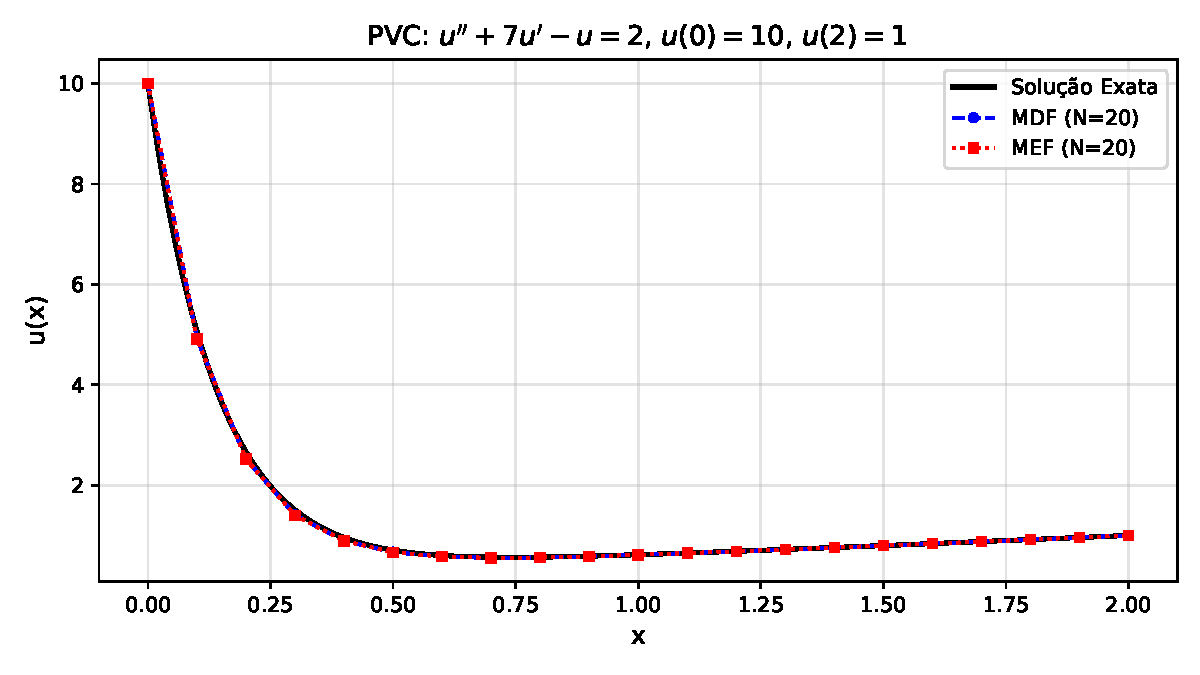
\includegraphics[width=0.88\textwidth]{plot_unidade5.pdf}
\caption{Comparação entre MDF, MEF e solução exata no problema de difusão-convecção-reação.}
\end{figure}

%==========================================================
\section{Conclusão}
%==========================================================
A Unidade~5 completa o panorama metodológico de Métodos Numéricos~II com a abordagem de problemas estacionários. Enquanto o MDF discretiza a formulação forte com estênceis de diferenças centrais — simples de implementar e de analisar —, o MEF parte da formulação fraca de Galerkin, que acomoda naturalmente condições de Neumann e domínios complexos.

Os experimentos confirmaram que ambos os métodos, para $\mathrm{Pe}_h < 1$, são estáveis e de segunda ordem em malhas uniformes. O MDF 2D com Gauss-Seidel preservou a simetria física esperada na equação de Poisson. O gráfico gerado em \texttt{matplotlib} e embutido no relatório evidencia a excelente aderência de ambos os esquemas à curva analítica, com desvios expressivos apenas na camada limite junto a $x=0$.

\end{document}
